% !TeX spellcheck = cs_CZ
%{\tikzset{external/prefix={tikz/FYZII/}}
% \tikzset{external/figure name/.add={ch39_}{}}
%---------------------------------------------------------------------------------------------------
% file fey2ch39.tex
%---------------------------------------------------------------------------------------------------
%=========================== Kapitola Pružné látky =================================================
\chapter{Pružné látky}\label{fyz:IIchapIXL}
\minitoc
  \section{Tenzor deformace}\label{fyz:IIchapIXLsecI}
  \section{Tenzor pružnosti}\label{fyz:IIchapIXLsecII}
  \section{Pohyby v pružném tělese}\label{fyz:IIchapIXLsecIII}
  \section{Nepružné chování}\label{fyz:IIchapIXLsecIV}
  \section{Výpočet konstant pružnosti}\label{fyz:IIchapIXLsecV}

    \begin{figure}[ht!]
      \centering
      \begin{tabular}{c}
        \subfloat[ ]{\label{fyz_fig788a}
          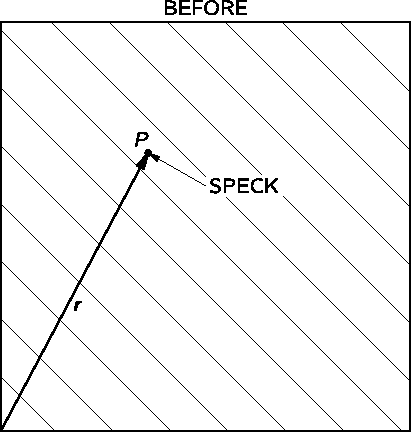
\includegraphics[width=0.7\linewidth]{fyz_fig788a.pdf}}               \\
        \subfloat[ ]{\label{fyz_fig788b}
          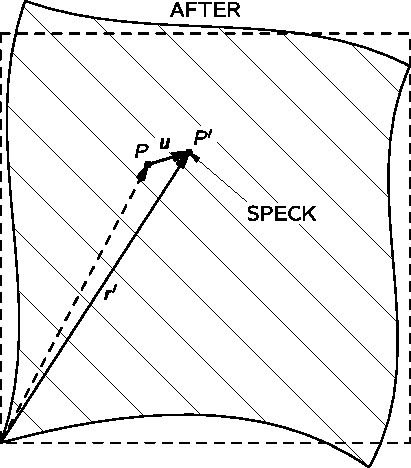
\includegraphics[width=0.7\linewidth]{fyz_fig788b.pdf}}
      \end{tabular}
      \label{fyz_fig788}
      \caption{
               (\cite[s.~748]{Feynman02})}
    \end{figure}

    \begin{figure}[ht!] %\ref{fyz_fig789}
      \centering
      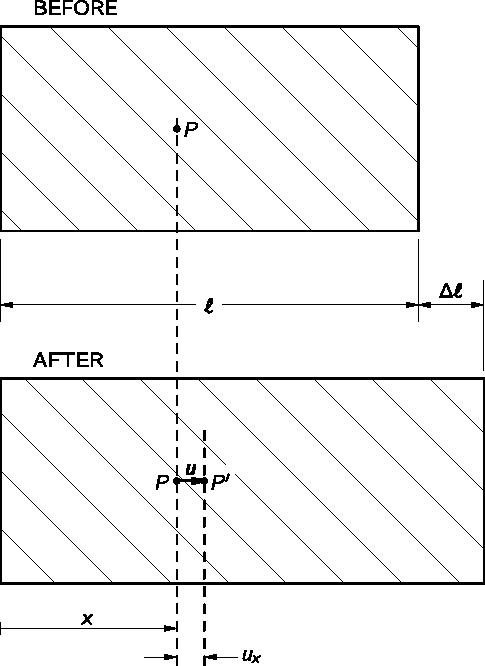
\includegraphics[width=0.7\linewidth]{fyz_fig789.pdf}
      \caption{
               (\cite[s.~707]{Feynman02})}
      \label{fyz_fig789}
    \end{figure}

    \begin{figure}[ht!]
      \centering
      \begin{tabular}{c}
        \subfloat[ ]{\label{fyz_fig790a}
          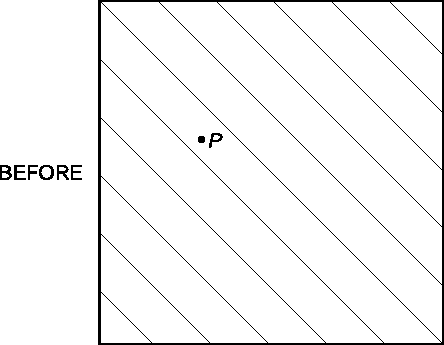
\includegraphics[width=0.7\linewidth]{fyz_fig790a.pdf}}               \\
        \subfloat[ ]{\label{fyz_fig790b}
          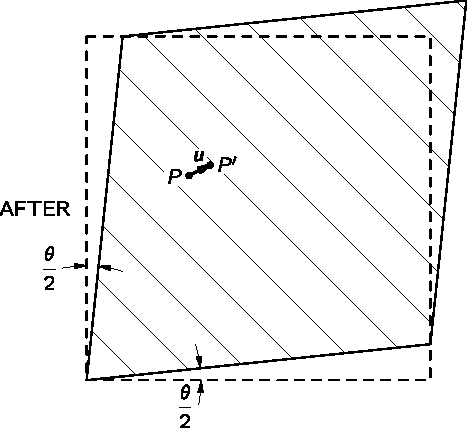
\includegraphics[width=0.7\linewidth]{fyz_fig790b.pdf}}
      \end{tabular}
      \label{fyz_fig790}
      \caption{
               (\cite[s.~748]{Feynman02})}
    \end{figure}

    \begin{figure}[ht!]
      \centering
      \begin{tabular}{c}
        \subfloat[ ]{\label{fyz_fig791a}
          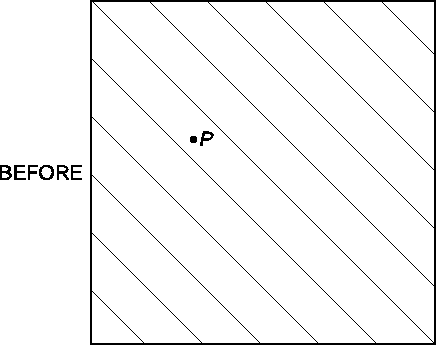
\includegraphics[width=0.7\linewidth]{fyz_fig791a.pdf}}               \\
        \subfloat[ ]{\label{fyz_fig791b}
          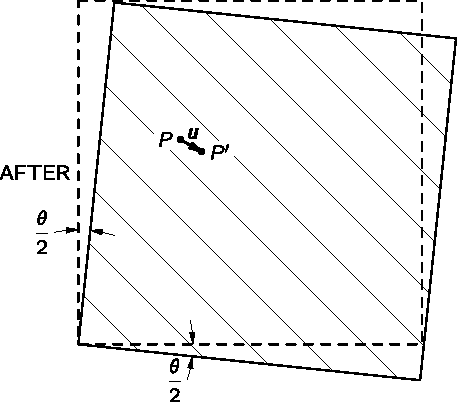
\includegraphics[width=0.7\linewidth]{fyz_fig791b.pdf}}
      \end{tabular}
      \label{fyz_fig791}
      \caption{
               (\cite[s.~748]{Feynman02})}
    \end{figure}

    \begin{figure}[ht!] %\ref{fyz_fig792}
      \centering
      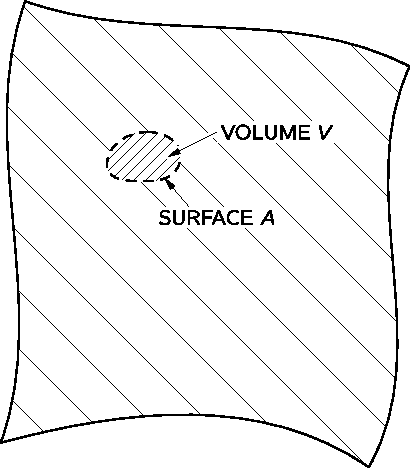
\includegraphics[width=0.7\linewidth]{fyz_fig792.pdf}
      \caption{
               (\cite[s.~707]{Feynman02})}
      \label{fyz_fig792}
    \end{figure}

    \begin{figure}[ht!] %\ref{fyz_fig793}
      \centering
      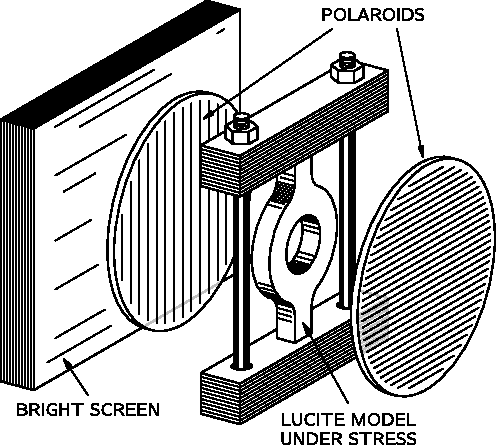
\includegraphics[width=0.7\linewidth]{fyz_fig793.pdf}
      \caption{
               (\cite[s.~707]{Feynman02})}
      \label{fyz_fig793}
    \end{figure}

    \begin{figure}[ht!] %\ref{fyz_fig794}
      \centering
      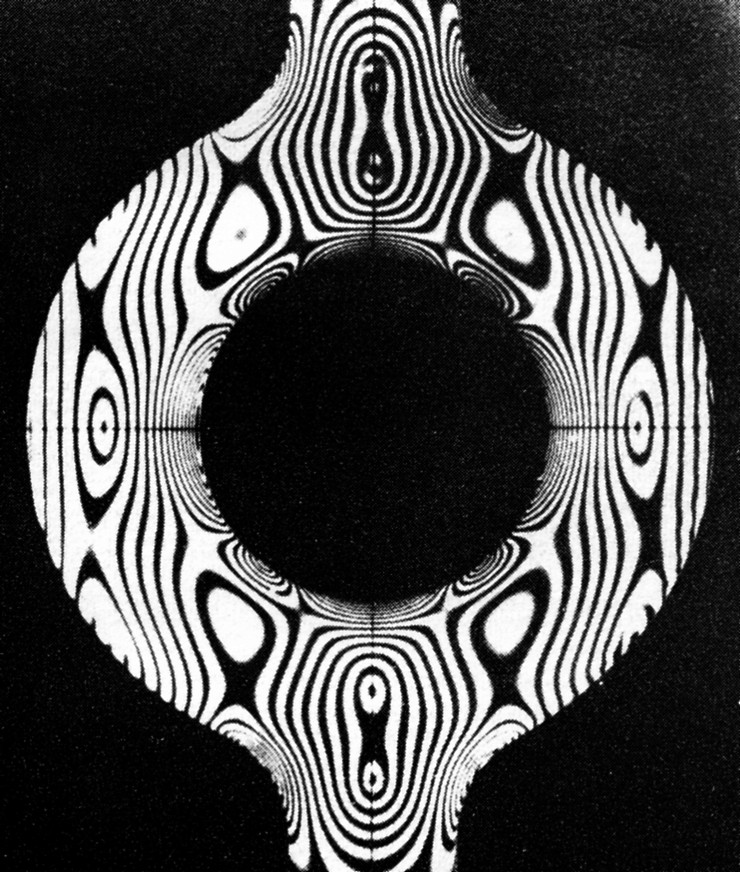
\includegraphics[width=0.7\linewidth]{fyz_fig794.jpg}
      \caption{
               (\cite[s.~707]{Feynman02})}
      \label{fyz_fig794}
    \end{figure}

    \begin{figure}[ht!] %\ref{fyz_fig795}
      \centering
      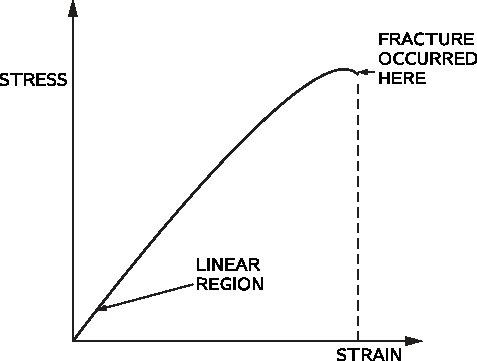
\includegraphics[width=0.7\linewidth]{fyz_fig795.pdf}
      \caption{
               (\cite[s.~707]{Feynman02})}
      \label{fyz_fig795}
    \end{figure}

    \begin{figure}[ht!]
      \centering
      \begin{tabular}{c}
        \subfloat[ ]{\label{fyz_fig796a}
          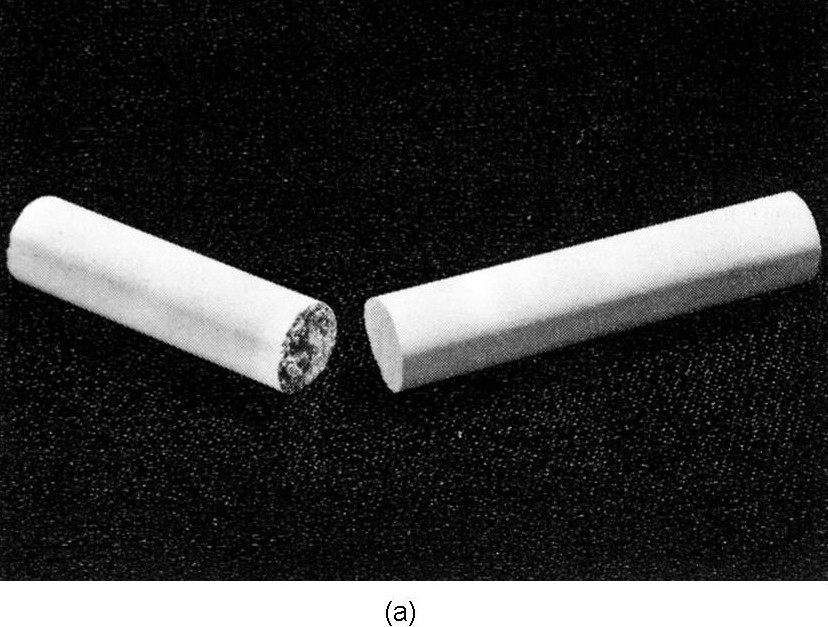
\includegraphics[width=0.7\linewidth]{fyz_fig796a.jpg}}               \\
        \subfloat[ ]{\label{fyz_fig796b}
          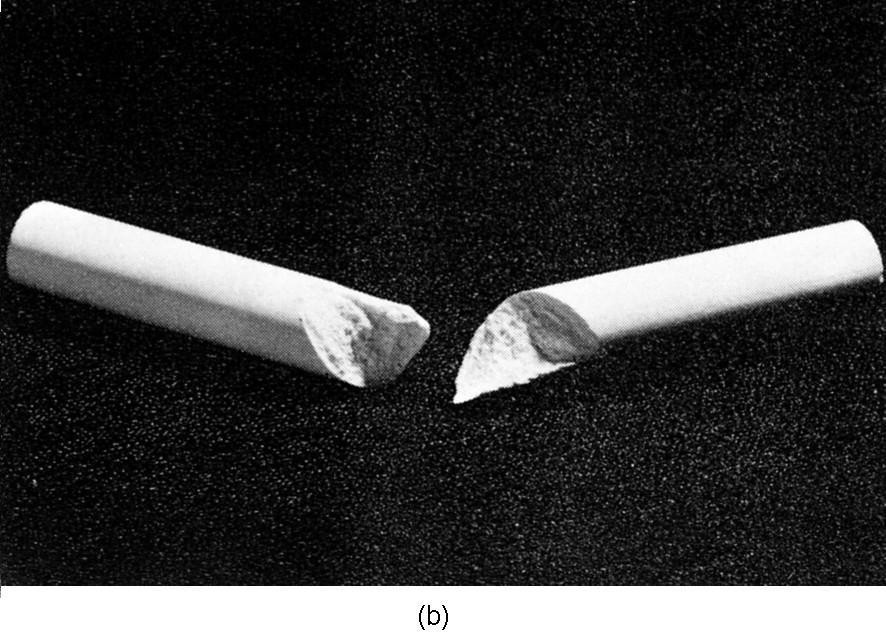
\includegraphics[width=0.7\linewidth]{fyz_fig796b.jpg}}
      \end{tabular}
      \label{fyz_fig796}
      \caption{
               (\cite[s.~748]{Feynman02})}
    \end{figure}

    \begin{figure}[ht!]
      \centering
      \begin{tabular}{c}
        \subfloat[ ]{\label{fyz_fig797a}
          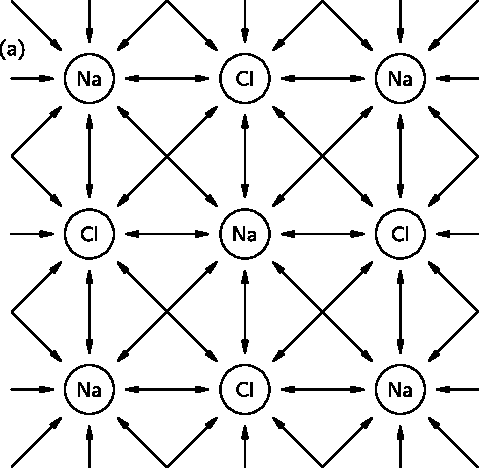
\includegraphics[width=0.7\linewidth]{fyz_fig797a.pdf}}               \\
        \subfloat[ ]{\label{fyz_fig797b}
          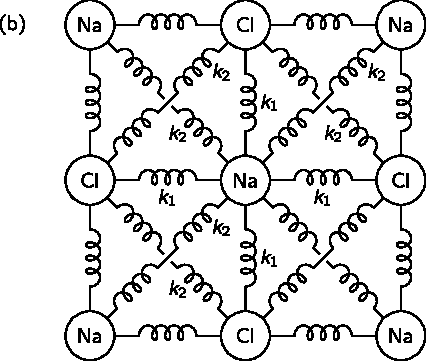
\includegraphics[width=0.7\linewidth]{fyz_fig797b.pdf}}
      \end{tabular}
      \label{fyz_fig797}
      \caption{
               (\cite[s.~748]{Feynman02})}
    \end{figure}

    \begin{figure}[ht!] %\ref{fyz_fig798}
      \centering
      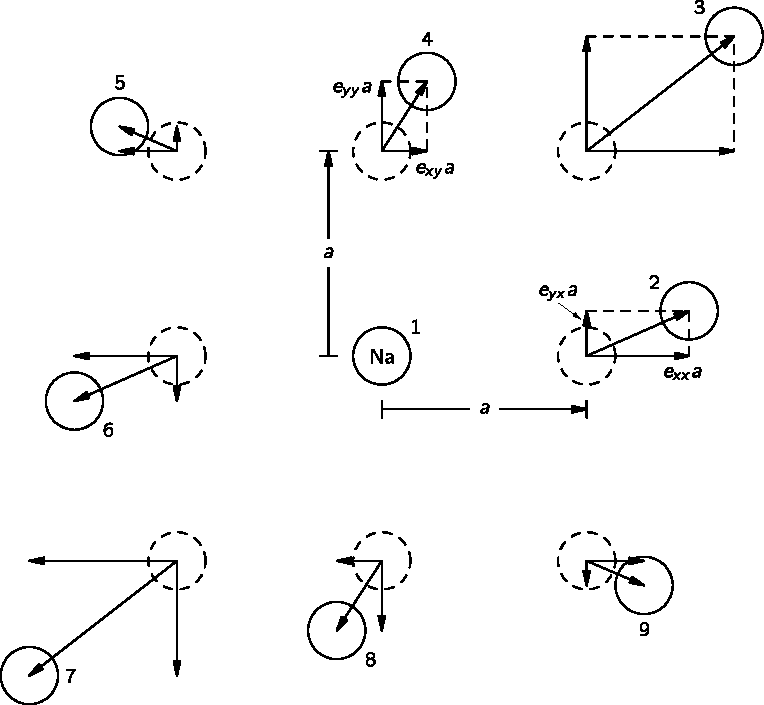
\includegraphics[width=0.7\linewidth]{fyz_fig798.pdf}
      \caption{
               (\cite[s.~707]{Feynman02})}
      \label{fyz_fig798}
    \end{figure}

%} %tikzset
%---------------------------------------------------------------------------------------------------
%\printbibliography[title={Seznam literatury},heading=subbibliography]
\addcontentsline{toc}{section}{Seznam literatury}